\documentclass[a4paper, 15pt]{article}
\usepackage[left=0.85in, right=0.85in, top=0.5in, bottom=0.95in]{geometry}
\usepackage[T1]{fontenc}
\usepackage[utf8]{inputenc}
\usepackage[italian]{babel}

% Formattazione del testo
\usepackage{setspace}         % Setting dello spazio\begin{spacing}{0.95}
\setstretch{1.2}
\setlength{\parindent}{0pt}
\raggedbottom
\usepackage[none]{hyphenat}    % no sillabazione 
\usepackage{multicol}          % testo su più colonne
\usepackage{changepage}	       % \begin{adjustwidth}{}{}

% Matematica
\usepackage{amsmath, amssymb, amsthm, mathtools}
\usepackage{cancel}            % semplificazioni \cancel{expression}
\newtheorem*{thm}{Teorema}
\newtheorem*{en}{Enunciato}
\newtheorem*{definizione}{Definizione}
\newtheorem*{cor}{Corollario}
\DeclareMathOperator{\rk}{rk}
\DeclareMathOperator{\im}{Im}
\DeclareMathOperator{\ev}{ev}

% Simboli e Disegni
\usepackage{color}             % \textcolor{'ColorCode'}{'testo'}
\usepackage{graphicx, wrapfig, float}
\usepackage{fancyhdr}
\usepackage{tikz, circuitikz, tkz-euclide}
\usetikzlibrary{patterns, arrows, decorations.markings, arrows.meta, decorations.text}
\tikzset{immagine/.style={above right, inner sep=0pt, outer sep=0pt},
testo/.style={fill=white, align=center, fill opacity=0.6, text opacity=1, below, font=\sffamily\bfseries\footnotesize}}
\usepackage{pgfplots}
\pgfplotsset{compat=1.15}
\usepackage{mathrsfs}

% Altri pacchetti
\usepackage{enumitem}
\usepackage{mdwlist} 	       % suspend enumerate \suspend{} \resume{}
\usepackage{siunitx}
\usepackage{hyperref}
\hypersetup{
colorlinks=true,
linkcolor=blue,    
urlcolor=blue,
}
\urlstyle{same}

% Altre definizioni personali
\usepackage{pifont}
\newcommand{\cmark}{\ding{51}}
\newcommand{\xmark}{\ding{55}}
\DeclareUnicodeCharacter{20AC}{\EUR}
\newcommand{\compresslist}{\setlength{\itemsep}{1pt}\setlength{\parskip}{0pt}\setlength{\parsep}{0pt}}
\newcommand{\ra}[1]{\renewcommand{\arraystretch}{#1}} % stretcho le tabelle e gli array \ra{x}
\setlength{\jot}{10pt}

%=======HEADER & FOOTER=======%
\def\lesson{Lezione N.27}


\pagestyle{fancy}
\fancyhf{}
\renewcommand{\headrulewidth}{0pt}
\renewcommand{\footrulewidth}{1.4pt}
\lfoot{A.M. $\diamond$ \the\year}
\cfoot{\thepage}
\rfoot{\lesson}


% Titolo e data
\title{Parte 19: ruote cilindriche a denti elicoidali}
\date{}

\begin{document}
\maketitle
\setcounterpageref{secnumdepth}{0}
\setcounter{tocdepth}{5}  % Includo nel TOC anche i subsubpar	
\tableofcontents 
\newpage



%\end{adjustwidth}
%\newpage
\section{Ruote cilindriche con denti elicoidali}
\begin{adjustwidth}{2in}{}
		Le ruote cilindriche elicoidali sono, da un certo punto di vista, un'ottimizzazione di quelle cilindriche a denti dritti, sfruttando un'intuizione che consiste nel sviluppare il profilo del fianco del dente attraverso un'estrusione non più assiale, ma lungo un'elica che si avvolge lungo la circonferenza fondamentale. \newline 
		
		Tale ruota dentata si può vedere anche, in prima approssimazione, come un numero finito di ruote dentate a denti dritti di spessore assiale molto piccolo, che vengono ruotate una rispetto all'altra di un angolo fisso: ogni "fettina" è stata ruotata lungo un angolo ottenendo un profilo a gradino. 
		\begin{figure}[H]
			\centering
			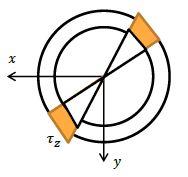
\includegraphics[width=0.5\linewidth]{figures/screenshot001}
			\label{fig:screenshot001}
		\end{figure}
		La ruota in immagine si chiama Ruota di Hooke ed è quindi Si definisce ruota di Hooke quella ruota che si ottiene a partire da una ruota a denti dritti dividendola, mediante
		piani perpendicolari all’asse, in tante fette di spessore costante e facendole ruotare le une rispetto alle altre di un
		angolo anch’esso costante.\newline 
		
	 	\textbf{Piano frontale/Trasversale}: piano in cui sono individuabili i denti dritti ed un profilo esattamente ad evolvente. 
	 	
	 	In questo piano sono facilmente individuabili la circonferenza primitiva, quella di testa, quella di piede e delle troncature esterna e interna.  
	 	\begin{figure}[H]
	 		\centering
	 		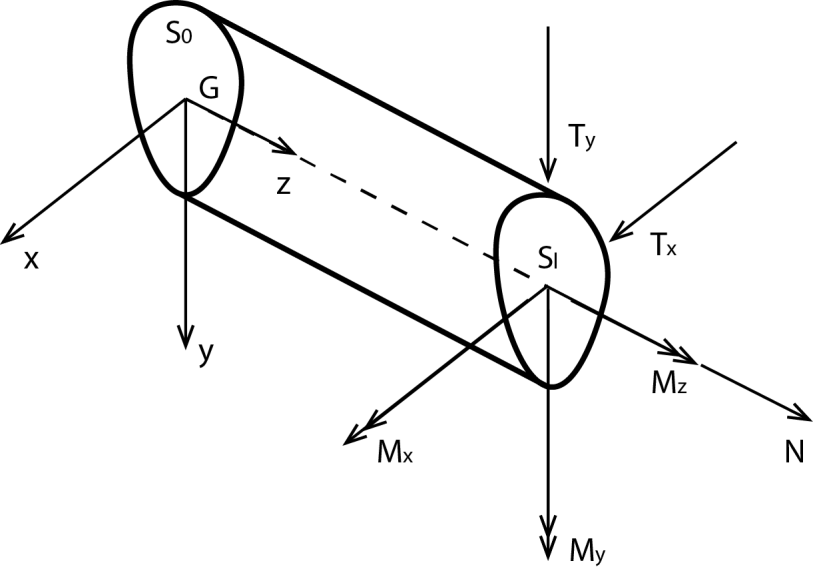
\includegraphics[width=0.5\linewidth]{figures/screenshot002}
	 		\label{fig:screenshot002}
	 	\end{figure}	 	
	 	Il profilo del dente si estende tridimensionalmente seguendo l'elicoide, il fianco del dente è in contatto con il suo coniugato lungo la linea dei contatti, che ora non sarà più assiale come nel caso dei denti dritti, la diventerà inclinata. \newline 
		
		Nell'accoppiamento necessariamente l'elica dev'essere di verso opposto tra motrice e condotta, per cui si sceglieranno un'elica sinistra e un'elica destra per pignone e ruota o viceversa. \newline 
		
		Si immagini di estendere il raggio di curvatura della primitiva di una ruota e portarla a curvatura infinita, ecco così che si viene di nuovo a formare un accoppiamento ruota/rocchetto - dentiera. 
		
		Che differenza c'è ora tra la dentiera così creata e quella che si aveva nel caso di denti dritti? 
		\begin{figure}[H]
			\centering
			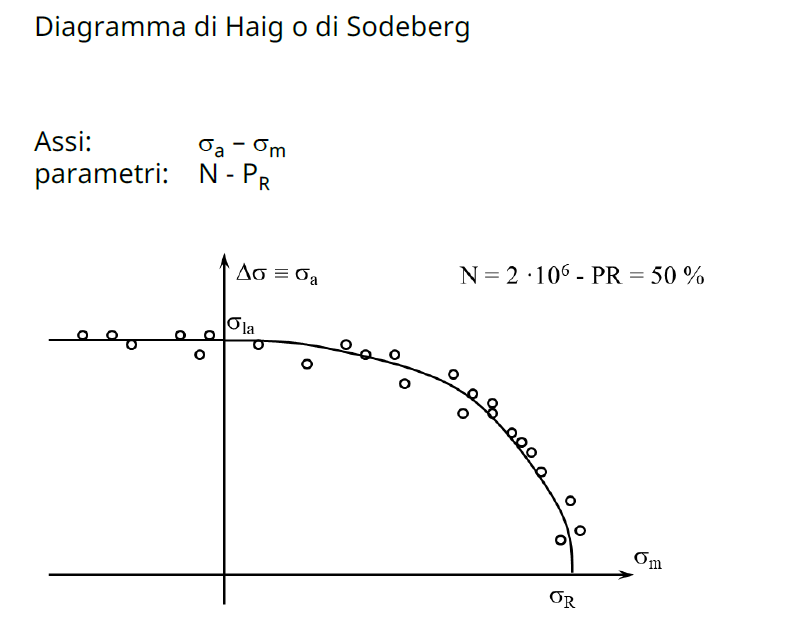
\includegraphics[width=0.5\linewidth]{figures/screenshot003}
			\label{fig:screenshot003}
		\end{figure}
		La dentiera presenta un'inclinazione d'elica $\alpha$.  
\newpage		
		Il cilindro di base della ruota dentata è sempre quello con raggio $\rho$, si immagini poi di avere un piano tangente a tale circonferenza fondamentale, la sezione di questo accoppiamento sul piano frontale è esattamente la retta dei contatti analizzata per le ruote dentate a denti dritti. 
		\begin{figure}[H]
			\centering
			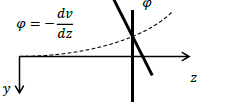
\includegraphics[width=0.3\linewidth]{figures/screenshot004}
			\label{fig:screenshot004}
		\end{figure}
		Se si considera ora una retta $a$ inclinata di un certo $\alpha_f$ rispetto alla direzione dell'asse, questa retta rappresenterà l'intersezione tra il piano dei contatti e il fianco del dente della dentiera. 
		
		In pratica se si avvolge questo piano  sulla circonferenza fondamentale, la superficie descritta dalla retta $a$, rappresenta  il fianco del dente elicoidale. 
		
		Esattamente come è stato spiegato nella ruota dentata a denti dritti, solo che su quel piano c'era una retta orientata come l'asse e poi non si era nemmeno parlato di rette, ma di punti, perché nella ruota dentata a denti dritti ci si limitava a guardare il piano frontale e si osservava che un punto sul piano dei contatti, avvolto sulla circonferenza fondamentale generava un'evolvente.  \newline 
		
		Dire che il profilo del dente dritto era un'estrusione assiale equivaleva a dire che esistevano infiniti punti allineati assialmente con questo punto frontale che facevano lo stesso percorso, lasciando l'impronta del dente ad evolvente assialmente dritta. \newline 
		
		\underline{ORA} se i punti dietro al piano frontale anziché essere perfettamente assialmente disposti, fossero tutti lungo una retta $a$ inclinata di un angolo $\alpha_f$, la forma che assume il dente è quella elicoidale, ed il profilo del dente avrà sviluppo elicoidale. \newline 
		
		L'elica lungo la quale si avvolge il profilo del dente non è altro che l'importa sulla circonferenza fondamentale di questa rulletta, cioè quando la retta $a$ si avvolge sulla circonferenza fondamentale e arriva alla fine a toccare tutta, descrive sul cilindro fondamentale un'elica. 
		
		Di quest'elica diventa così possibile scrivere il passo $h$, cioè la distanza assiale che quest'elica compie dell'effettuare un completo giro di circonferenza 
		\[\dfrac{2\pi\rho}{h} = \tan\alpha_f\]
		Dove $\alpha$ è l'angolo d'elica ed il pedice $f$ indica che viene misurato sulla circonferenza fondamentale.  
\newpage		
		Per come è stata fin'ora costruita, sul piano frontale, la forma del dente sarà - come detto - perfettamente ad evolvente ed in qualunque sezione trasversale, si individuerà sempre lo stesso profilo ad evolvente, ciò permette facilmente di affermare che sono ancora valide tutte le proprietà dei profili ad evolvente coniugati: il cinematismo avviene sempre come rotolamento senza strisciamento di ude circonferenza primitive  che ruotano intorno all'asse ortogonali al piano frontale.   
\end{adjustwidth}
%\newpage
\section{Alcune proprietà}
\begin{adjustwidth}{2in}{}	
	\begin{itemize}
		\item L’elicoide ad evolvente è una superficie rigata costituita dalle posizioni successive della retta generatrice $a$, o ugualmente, per ogni punto della sua superficie passa una retta di tipo $a$. \newline 
		
		Questa superficie di fianco si ottiene considerando le posizioni di inviluppo delle posizioni successive  della retta $a$ durante l'avvolgimento dell'evolvente. 
		
		\item Se si prende un generico punto P sull'elicoide, allora il piano tangente in P, intersecato con  il piano tangente alla circonferenza fondamentale, genera la retta $a$. \newline 
		
		L'intersezione tra il piano tangente alla fondamentale e il piano tangente al profilo del dente passante per un generico punto P, avviene ortogonalmente e la loro intersezione è la retta $a$ inclinata di un angolo $\alpha_f$. 
		\begin{figure}[H]
			\centering
			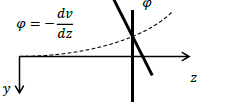
\includegraphics[width=0.7\linewidth]{figures/screenshot004}
			\label{fig:screenshot004.1}
		\end{figure}
		Il fatto che siano ortogonali vuol dire che la normale al punto P giace in quel piano inclinato tangente alla fondamentale e questo è vero per qualsiasi punto P appartenente alla retta $a$ e per qualunque retta $a$ appartenente alla superficie rigata del fianco  dell'elicoide. 
		
		Questo vuol dire che:   
		
		\item La normale $\hat{n}$ alla superficie dell'elicoide giace/è contenuta nel piano tangente al cilindro fondamentale passante per P ed è normale alla retta $a$ per P. 
		
		Ovvero la normale al profilo in un punto giace su questo piano tangente, che sarà il piano contenente la retta d'azione. \newline 
		
		Siccome vigono tutte le proprietà dell'evolvente si può così dire che quel piano sarà anche il piano contenente i punti di contatto, proprio perché per proprietà dell'evolvente per quel punto P ci potrà essere il coniugio di un'altra ruota dentata, cioè due profili coniugati che si toccano secondo proprietà dell'evolvente con normale in comune contenuta nel piano inclinato e quindi quello sarà il piano dei contatto della ruota dentata elicoidale. \newline 
		
		Il segmento dei contatti non è più una retta assiale  di larghezza pari a quella di fascia, ma sarà un segmento inclinato, esattamente la retta $a$.  
		
		\item  Il piano ortogonale a questo piano inclinato, $\gamma$ tangente al profilo dell'elicoide, rappresenta il fianco  del dente della dentiera che ha scavato la ruota dentata. 		
	\end{itemize}	
\end{adjustwidth}
%\newpage
\section{Raggi di curvatura}
\begin{adjustwidth}{2in}{}	
Parlando di ruote dentate a denti dritti ci si era posti il problema di cosa accadeva sul piano frontale caratterizzando la superficie del dente soltanto su quel piano. 

In realtà il fianco del dente - anche nella ruota dentata a denti dritti - è una superficie a doppia curvatura, come tutte le superfici tridimensionali, solo che - com'è noto - una superficie tridimensionale ha in ogni punto ha una coppia di raggi di curvatura almeno due tra loro principali (non c'è torsione della geometria) e nel caso di ruota dentata a denti dritti, le curvature  si tracciavano considerando in un punto le circonferenze osculatrici in una direzione e nella sua direzione ortogonale. 

Sempre per i denti dritti, una curvatura principale è quella che passa nel punto P secondo una traccia assiale. 

\begin{figure}[H]
	\centering
	\begin{tikzpicture} [>=latex]
	%%%	Help Lines
%	\draw [thin, help lines] (0,0) grid (10,5);
%	\foreach \x in {0,...,10}
%	\draw (\x cm,1pt) -- (\x cm,-1pt) node[anchor=north] {$\x$};
%	\foreach \y in {0,...,5}
%	\draw (1pt,\y cm) -- (-1pt,\y cm) node[anchor=east] {$\y$};
	%%%	Disegno	
	\draw[thick] (1,0) arc (180:100:1.25 and 2.5);
	\draw[thick] (4,0) arc (0:80:1.25 and 2.5);
	\draw[thick] (1,0) -- (4,0);
	\draw[thick] (2,2.46) -- (3,2.46);
	\draw[thick] (3,2.46) -- (6,4.46); 
	\draw[thick] (2,2.46) -- (5,4.46); 
	\draw[thick] (5,4.46) -- (6,4.46);
	\draw[thick] (7,2) arc (0:80:1.25 and 2.5);
	\draw[thick] (4,0) -- (7,2);
	\draw[thick, red] (5.5,1.75) arc (30:70:1.25 and 2.5);
	\draw[thick, blue] (4.75,2) -- (5.75,2.75);
	\node[red] at (5.25, 2.75) {P};	
\end{tikzpicture}
\end{figure} 

In un punto P si avranno due curvature, cioè la rigatura  della superficie si deve approssimare con dei raggi di curvatura:
\begin{itemize}
	\item Una \textcolor{blue}{curvatura} principale sarà rettilinea e quindi avrà raggio di curvatura $\infty$
	
	\item L'altra \textcolor{red}{curvatura} principale nel piano ortogonale (nel piano frontale passante per P) varrà per Eulero-Savary - se quel punto è di contatto - come la distanza sul piano  del contatti dal punto dei contatti fino ad $\Omega$, centro di curvatura o punto di tangenza del piano dei contatti con la circonferenza fondamentale
\end{itemize} 
	In una rappresentazione bidimensionale:	
	\begin{figure}[H]
		\centering
		\begin{tikzpicture}[scale=.75]
		%%%	Help Lines
%		\draw [thin, help lines] (0,0) grid (10,10);
%		\foreach \x in {0,...,10}
%		\draw (\x cm,1pt) -- (\x cm,-1pt) node[anchor=north] {$\x$};
%		\foreach \y in {0,...,10}
%		\draw (1pt,\y cm) -- (-1pt,\y cm) node[anchor=east] {$\y$};
		
		%%% Punti
		\tkzDefPoints{8/6/omega1, 5/4/P, 5/10/C1, 5/1/C, 5/5/R1, 5/3.5/R}		
		\node [right] at (P) {$P$};		% Punto di contatto
		\node [right] at (C1) {$C'$}; 	% Centro condotta
		\node [right] at (C) {$C$};		% Centro motrice
		
		%%%	Disegno	
		\draw[thick] (10,10) arc (0:-180:5);
		\draw[thick] (2.5,1) arc (180:0:2.5);
		%	\tkzDrawCircles(C1,R1 C,R)
		
		
		%%% Calcolo dei punti di tangenza
		\tkzDefTangent[from = P](C1,R1) \tkzGetPoints{T1a}{T1b}
		\tkzDefTangent[from = P](C,R) \tkzGetPoints{T2a}{T2b}
		% Questo comando calcola i punti di tangenza tra la circonferenza C1 e una retta passante per il punto P. I punti di tangenza vengono memorizzati in T1a e T1b.
		
		%%% Disegno della tangente
		\draw[red, thick] (P) -- ($(P)!1.5!(T1b)$) node[right] {$\Omega'$};
		\draw[red, thick] (P) -- ($(P)!1.5!(T2b)$) node[left] {$\Omega$};
		% Questo comando disegna la tangente dalla posizione di P al punto di tangenza % T1a sulla circonferenza C1. La parte ($(P)!1.5!(T1a)$) calcola un punto lungo la retta da P a T1a a una distanza del 150% dalla lunghezza della 
		% retta.
		\tkzDrawPoints (T1b,T2b,P, C, C1)
	\end{tikzpicture}
	\end{figure}	
	$P\Omega$ è il raggio di curvatura, così come per profilo coniugato, $P\Omega'$. 
	
	Questi erano i raggi di curvatura per i profili a denti dritti. \newline 
	
	Si vuole ora ripetere lo stesso ragionamento ma su un profilo a denti elicoidali dove la superficie è a doppia curvatura e si svolge lungo l'elicoide.
	
	\begin{proof}
		Si immagini di avere una superficie generica sulla quale si individua il punto P. 
		
		Nello stesso punto si individui una retta tangente alla superficie $u$. 
		
		Si immagini poi di individuare alcune delle infinite curve regolari che soddisfino le seguenti condizioni: essere tangenti ad $u$, passanti per P e giacenti sulla superficie $C, C_n$. 
		
		\begin{figure}[H]
			\centering
			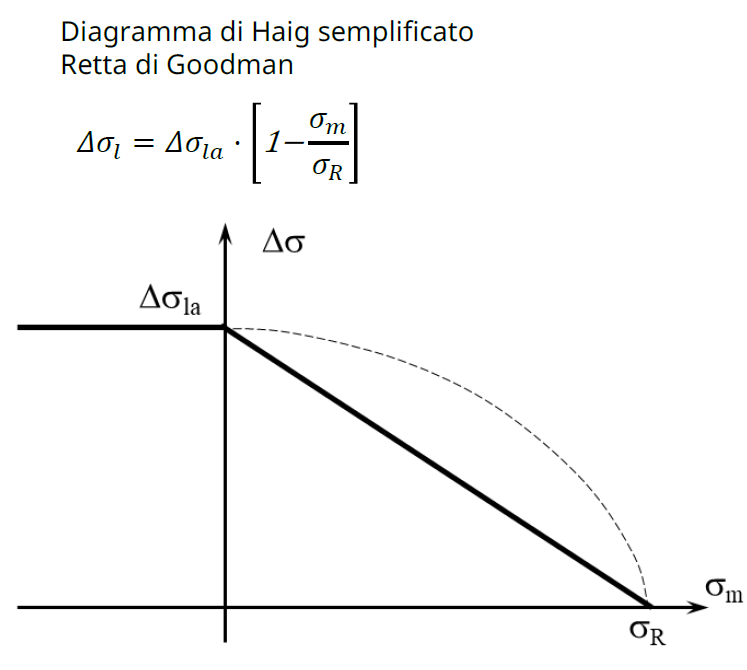
\includegraphics[width=0.35\linewidth]{figures/screenshot005}
			\label{fig:shot005}
		\end{figure}
		
		Queste curve regolari si ottengono per intersezione della superficie con dei piani che contengano $u$. e intersechino la superficie. 
		
		Sia $C_n$ quella particolare curva ottenuta dall'intersezione  della superficie con un piano contenente $u$ e la normale $\hat{n}$ alla superficie $\Sigma$ in P. 
		
		\textbf{Reminder:} il versore ortogonale alla superficie in P è unico. 
		
		Si trova così il piano $\sigma_n$ che contiene $\hat{n}$ ed $u$. \newline 
		
		Il raggio di curvatura della $C_n$ in P è pari a $R_n$.
		
		Si immagini ora di sezionare nuovamente la superficie con un piano $\sigma$ inclinato di un angolo $\varphi$ rispetto al piano $\sigma_n$ contenente sempre la direzione $u$: si ottiene ora una nuova curva di intersezione $C$. 
		
		In P il raggio di curvatura della curva C sarà necessariamente diverso dal raggio di curvatura della curva $C_n$ 
		\[R = R_n\cos\varphi \]
	\end{proof}

Il risultato di questa dimostrazione può essere utilizzato per lo studio del profilo dei denti elicoidali. 

Nel profilo di questa dentatura, in un qualsiasi punto P si possono sempre individuare due curvature principali. 

\begin{itemize}
	\item Una è ancora quella rettilinea: in un intorno infinitesimo del punto P quel segmento è rettilineo, anche perché segue la retta a, per definizione rettilinea inclinato di un angolo $\alpha_f$. 
	
	\item Per la seconda curvatura principale (quella ortogonale alla prima) il raggio di curvatura è necessariamente diverso da quello che si aveva nel profilo a denti dritti, infatti se si individua un piano normale al dente, cioè un piano che contenga la normale alla superficie nel punto P,  la curvatura in quel punto sarà l'$R_n$ della dimostrazione appena eseguita, e quindi si troverà a partire dal raggio di curvatura nel piano frontale (noto: raggio di curvatura del profilo ad evolvente $P\Omega$)
	\[\rho" = R_n = \dfrac{P\Omega}{\cos\alpha_f} = \dfrac{R\sin\theta + \delta}{\cos\alpha_f}\] 
	Dove si è usato 
	\[P\Omega = R\sin\theta + \delta\]	
	Questa curvatura così individuata sarà estremamente importante per valutare la resistenza del dente a profilo elicoidale. 
\end{itemize}	
\end{adjustwidth}
%\newpage
\section{Contatto}
\begin{adjustwidth}{2in}{}
		Nel caso della ruota dentata a denti dritti il contatto - su tutta la larghezza di fascia - iniziava quando la testa di una ruota toccava l'intorno del piede dell'altra. 
		
		Durante l'ingranamento  quel contatto poi si svolgeva lungo il profilo del dente, una dalla testa al piede a l'altra dal piede alla testa. 
		
		In una sezione trasversale si guardava il primo punto della linea di contatto (perché gli altri punti stavano perfettamente uno dietro l'altro) e quel punto si muoveva lungo il segmento dei contatti fino alla fine dell'ingranamento. 
		
		La velocità di  percorrenza della retta dei contatti da parte del punto era dettata da una velocità  pari alla velocità periferica misurata sulla circonferenza fondamentale. 
		
		Si parlava perciò di un punto dei contatti su un segmento dei contatti, riducendo il tutto ad un problema bidimensionale.  
		
		In realtà il contatto è tridimensionale: una serie di punti allineati (punto dei contatti) che si muove in un piano di contatto (segmento dei contatti) da un profilo all'altra dell'evolvente. \newline 
		
		\underline{ORA}, introducendo una rotazione sul piano frontale del profilo del dente, si osserva che il primo contatto non avviene più contemporaneamente su tutta la larghezza di fascia, ma esisterà una coppia di denti che inizia a toccarsi testa-piede soltanto in un punto.
		
		Il contatto poi proseguirà su un altro punto individuato da un segmento inclinato di $\alpha_f$, fino ad interessare tutta  la larghezza di fascia della ruota. 
		\begin{figure}[H]
			\centering
			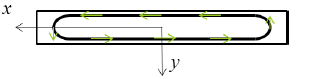
\includegraphics[width=0.7\linewidth]{figures/screenshot006}
			\caption{}
			\label{fig:screenshot006}
		\end{figure}
		(Guarda la figura e guarda le linee inclinate sul piano dei contatti, prima erano dritte e parallele all'unica retta AA', ora dato che la retta dei contatti è inclinata di un $\alpha_f$, le linee di progressivo contatti le cominci a tracciare da A inclinate di $\alpha_f$ e i punti discretizzati che individui, sono quelli di successivo contatto). \newline
		
		Questa linea dei contatti durante l'ingranamento si muoverà fino a ritornare un punto al termine dalla presa. 
		
		Quello che si osserva è un contatto progressivo, e questo spiega la silenziosità della ruota dentata a denti elicoidali rispetto a quella a denti dritti: il contatto inizia in un punto, si estende e poi si riduce, gli urti che ne scaturiscono sono ben minori. \newline
		
		Se si immaginasse di estrarre questa evoluzione del contatto sul piano dei contatti ribaltandolo di $90^\circ$, si ottiene l'effettiva rappresentazione del piano dei contatti. 
		
		Il movimento del segmento inclinato è di traslazione sul piano dei contatti con velocità periferica misurabile sulla circonferenza fondamentale, esattamente come per i denti dritti; questo perché ciascun punto di questa linea di contatto segue le modalità di movimento dall'evolvente in ua direzione ortogonale alla rappresentazione fornita.
		
		L'estensione di questa superficie va dalla troncatura esterna di una ruota alla troncatura esterna dell'altra.\newline 
		
		Una ruota dentata a denti elicoidali è diversa soltanto nella realizzazione, il suo funzionamento è identico a quelle a denti elicoidali. \newline 
		
		L'estensione della linea sul fianco che partecipa al contatto dipende dalle proporzione della ruota, se per una ruota dentata è sempre $b$ e corrisponde alla larghezza di fascia e cioè la dimensione assiale della ruota, per i denti elicoidali dipende dalla proporzione tra l'angolo $\alpha_f$ e le proporzioni assiali della ruota.
		\begin{figure}[H]
			\centering
			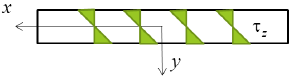
\includegraphics[width=0.5\linewidth]{figures/screenshot007}
			\caption{}
			\label{fig:screenshot007}
		\end{figure}		
		Infatti  
		\[\begin{dcases}
		(\delta_1+\delta_2)\cot\alpha_f>b \qquad \Rightarrow\qquad l_{max} = \dfrac{b}{\cos\alpha_f} \\
		(\delta_1+\delta_2)\cot\alpha_f<b \qquad \Rightarrow\qquad l_{max} = \dfrac{\delta_1+\delta_2}{\sin\alpha_f}
		\end{dcases}\] 
		Dove $\delta_1+\delta_2$ altri non è che la formulazione del segmento effettivo dei contatti: la distanza sul piano dei contatti tra lle due troncature esterne delle ruote. \newline 
		
		Per come è costruita, l'angolo d'elica che interessa dal punto di vista della rappresentazione geometrica dell'elicoide è $\alpha_f$: si realizza il profilo del dente avvolgendo la retta $a$ intorno ad una circonferenza fondamentale con passi $h$ definito da $\alpha_f$. \newline 
		
		Nella pratica però si hanno in mano tutte grandezze espresse sulla circonferenza primitiva (angolo di pressione, rapporto di trasmissione ...) e allora sarebbe molto più comodo avere un $\alpha_p$ riferito alla circonferenza primitiva piuttosto che a quella fondamentale. 
		
		Tuttavia
		\[\alpha_p\ne\alpha_f\]
		Imponendo il medesimo passo $h$, ovvero quella distanza che permette di effettuare un giro completo dell'elica, allora si vede subito si sta avvolgendo l'elica su di una circonferenza più grande. 
		\begin{figure}[H]
			\centering
			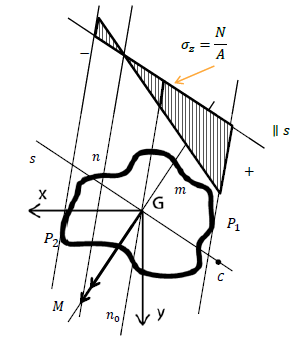
\includegraphics[width=0.5\linewidth]{figures/screenshot008}
			\label{fig:screenshot008}
		\end{figure}
		Quindi per ottenere lo stesso avvolgimento su questa circonferenza più grande, l'angolo dovrà essere differente. 
		
		Si ottiene così, chiamando per semplicità $\alpha=\alpha_p$
		\[2\pi\rho\cot\alpha_f = 2\pi R\cot\alpha\]
		Per cui, ricordando che $\rho = R\cos\theta$
		\[\tan\alpha_f = \tan\alpha\cos\theta\]
		Il cinematismo è basato su $\alpha_f$ mentre sul datasheet della ruota viene riportato $\alpha$. \newline 
		
		Tra le migliorie delle ruote dentate elicoidali rispetto a quelle a denti dritti è che si ha una migliore ripartizione del carico, ma per quale motivo? 
		
		A partecipare al contatto sono ben più di due denti in presa, nei denti dritti tipicamente $\varepsilon= 1,2\div1,6$, con i denti elicoidali appena si verifica si possono avere in contemporanea molti più denti in presa. 
		
		Ciò risiede nel fatto che il fattore di ricoprimento può essere visto come la somma di due contributi: 
		\begin{enumerate}
			\item Rapporto di condotta frontale (d'evolvente)
			\[\varepsilon = \dfrac{\delta_1 + \delta_2}{p\cos\theta}\]
			Ovvero il rapporto tra l'arco d'azione ed il passo. 
			
			Già visto per le ruote a denti dritti, tiene conto dello sviluppo dell'evolvente sul piano frontale.
			
			\item Rapporto di condotta normale (d'elica)
			\[\varepsilon_\alpha = \dfrac{b\tan\alpha}{p}\]
			Questo è dettato dal fatto che anche quando finisce il segmento dei contatti frontalmente, il contatto prosegue posteriormente al piano frontale. 
		\end{enumerate}  

Con riferimento alla figura \ref{fig:screenshot007}, è preferibile la soluzione mostrata a sinistra perché si vede immediatamente che la ripartizione del carico interessa tutta la larghezza di fascia, con una soluzione di destra, la risultate di pressione risultanti diviene sbilanciata rispetto alla larghezza di fascia: tutta sul frontale all'inizio e poi tutta sul posteriore alla fine. 	
	
\end{adjustwidth}

\section{Numero minimo di denti}
\begin{adjustwidth}{2in}{}		
Nella ruota dentata a denti elicoidale la proporzione modulare della dentatura e di tutte le grandezze geometriche di cinematismo che ne conseguono, è proprio di un piano contenente la normale al profilo. 

Sul piano frontale si ha un proporzionamento non più modulare: è la sezione effettuata con un piano ortogonale al profilo che contiene il proporzionamento modulare, ed è il piano che contiene il cinematismo di taglio dell'evolvente. 	
\begin{figure}[H]
	\centering
	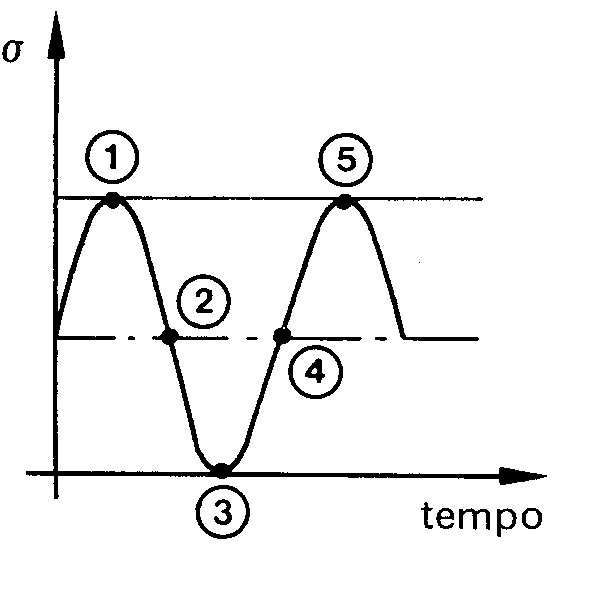
\includegraphics[width=0.5\linewidth]{figures/screenshot009}
	\label{fig:screenshot009}
\end{figure}
\textbf{ATTENZIONE}
\begin{itemize}
	\item Tutte le grandezze relative alla realizzazione della ruota dentata, quindi quelle associate ad in inviluppo della dentiera sul rocchetto,  si misurano sull'appena introdotto \textbf{piano normale}. 
	
	\item Tutte le grandezze relative al cinematismo dell'evolvente si misurano sul già noto \textbf{piano frontale/trasversale}. 
\end{itemize}

Le relazioni che si individuano così sul piano normale sono le relazioni che si individuavano per le ruote a denti dritti sul piano frontale. \newline 

Il piano $\gamma$ introdotto poco fa, passante per la retta $a$ e tangente al profilo, rappresenta proprio il  fianco del dente della dentiera, nient'altro che un dente inclinato appartenente ad una superficie di polare che è la stessa della dentiera della ruota dentata a denti dritti e si muove senza strisciare  avvolgendosi sulla circonferenza fondamentale del rocchetto. \newline 

Il modulo unificato della dentiera da $m_0$ diventerà $m_{0n}$. \newline

Che relazione c'è tra le grandezze misurate nel piano normale e quelle nel piano frontale? 

C'è una proporzione del tutto geometrica. 
\[\begin{dcases}
	p_n = p_f\cos\alpha\ \\
	m_n = m_f\cos\alpha \\	
\end{dcases}\]
Con $f$ ora pedice che indica il piano frontale. 

Il modulo normale è quello proprio della dentiera, quello che dimensiona il meccanismo di taglio, quello frontale si utilizzerà invece per verificare la resistenza del dente. \newline

 

Il proporzionamento della dentatura sarà diverso sul piano frontale e sul piano normale.

L’altezza del dente è sempre la stessa solamente che appare diversa, come proporzionamento, ad un osservatore
sul piano normale e ad uno sul piano frontale.

Mentre sul piano normale il dente ha una distanza tangenziale (distanza in direzione circonferenziale tra la testa ed il piede del dente) pari a 
\[w_f = (a+u)\tan\theta\]
Analogamente sul piano normale
\[w_n = (a+u)\tan\theta_n\]
Dove $\theta_n$ rappresenta l'angolo d'attacco della dentiera, non più l'angolo di pressione. 

Ora è sul piano frontale (senza pedice) che $\theta$ rappresenta l'angolo di pressione, e contribuisce a dare una forma diversa del dente, infatti essendo $w$ una dimensione lineare, vale sempre 
\[w_n = w_f\cos\alpha\]
Allora 
\[(a+u)\tan\theta_n = (a+u)\tan\theta\cos\alpha\]
Ottenendo infine la proporzione tra l'angolo d'accatto della dentiera misurato sul piano normale e l'angolo di pressione misurato sul piano frontale
\[\tan\theta_n = \tan\theta\cos\alpha\]

Per quale motivo non si usa parlare di "angolo di pressione" come si era fatto coi denti dritti? 

Perché in realtà il cinematismo di taglio non segue l'evolvente di circonferenza: il profilo del dente è sì ad evolvente sul piano frontale, ed è proporzionato modularmente nel piano normale, ma tale proporzionamento, dettato dall'accoppiamento con la dentiera, non genera un profilo del dente ad evolvente di circonferenza. 
\begin{figure}[H]
	\centering
	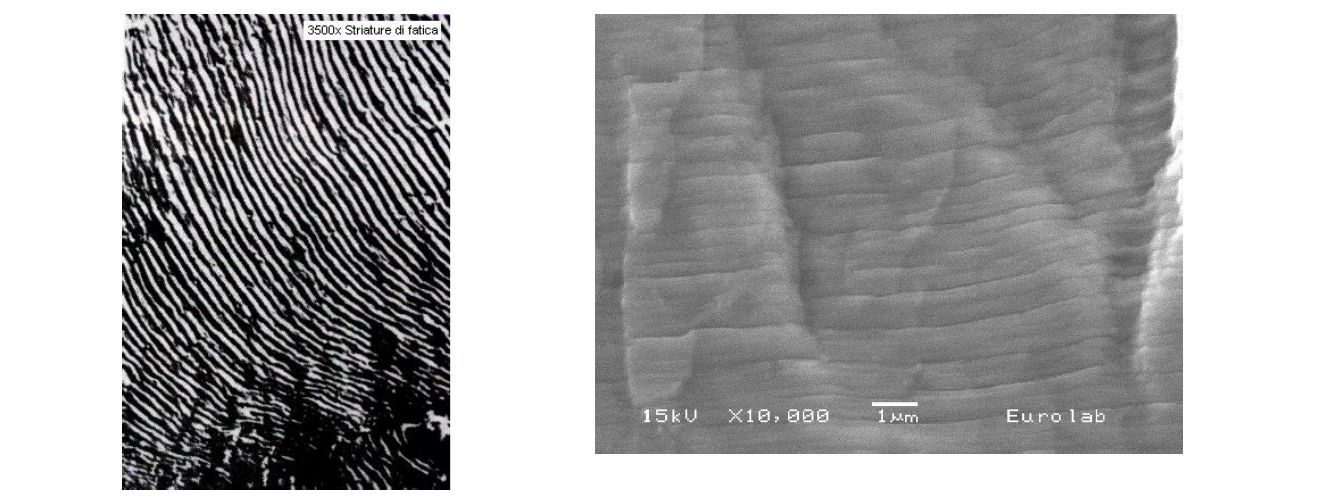
\includegraphics[width=0.25\linewidth]{figures/screenshot010}
	\caption{Sezione di piano normale}
	\label{fig:screenshot010}
\end{figure}
Questo perché sul cilindro fondamentale è stato avvolto un piano con asse NON ortogonale al piano normale. 

Sezionando infatti il piano normale si ottiene una retta (la traccia del piano contenente il piano fondamentale della dentiera) e un'ellisse: si è tagliato un cilindro con un piano inclinato. 

Nel piano normale si ha così un'evolvente di ellisse.

Poiché l'evolvente di ellisse ha proprietà differente dall'evolvente di circonferenza, si faranno della valide approssimazioni: nell'istante in cui i denti si stanno toccando nel punto P, in un piano normale l'accoppiamento potrebbe essere quello tra la retta appartenente al piano  della dentiera, ed una massima circonferenza $R^*$ tangente all'ellisse che ne approssimi la curvatura, fittizia. 

Si può così immaginare che il taglio avvenga come cinematismo d'accoppiamento tra un piano ed un cilindro $R^*$. \newline 

Ora quanto valgono i semiassi dell'ellisse? 
\[b'= R \qquad a'= \dfrac{R}{\cos\alpha}\]
Allora il raggio di curvatura della circonferenza fittizia considerata ai fini di questo ingranamento di taglio, sarà, per proprietà dell'ellisse
\[R^* = \dfrac{a'^2}{b'} = \dfrac{R}{\cos^2\alpha}\]
È come se si stesse realizzando una ruota dentata a denti dritti che abbia come primitiva di taglio una $R^*$. \newline 

Se questa dimensione fittizia però fosse reale, genererebbe una ruota fittizia di diametro primitivo pari ad $2R^*$ e quindi con un numero di denti fittizio pari a 
\[z^* = \dfrac{2R^*}{m_n} = \dfrac{2R}{m_n\cos^2\alpha} = \dfrac{2R}{m\cos^3\alpha} = \dfrac{z}{\cos^3\alpha} \]
Questa ruota fittizia altri non è che un'approssimazione istantanea dell'atto di taglio. 

Questa relazione evidenzia poi, quasi di sottecchi, il più grande vantaggio delle ruote a denti elicoidali: il numero minimo di denti che ne risulta è minore di quello di una ruota dentata a denti dritti ottenendo ingranaggi più compatti e prestazionali.

Tuttavia nell'inviluppo non si poteva andare sotto un certo numero di denti perché si manifesta troppa interferenza tra testa dentiera e base dente, ora però il problema dell'interferenza affligge solamente il numero di denti fittizio.\newline 

Quanto meglio ripartiscono il carico le ruote dentate elicoidali? 

Tornando indietro al fattore di ricprimento $\varepsilon$, questo è comporto da due fattori, il primo(d'evolvente) viaggia sempre intorno a valori di 1,5, il secondo (d'elica) darà invece il grosso del contributo, assumendo valori (per configurazioni molto spinte) prossimi a 30 e dipende linearmente dall'angolo d'elica $\alpha=\beta$.
\begin{figure}[H]
	\centering
	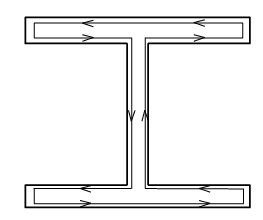
\includegraphics[width=0.5\linewidth]{figures/screenshot011}
	\label{fig:screenshot011}
\end{figure}
Valori troppo elevati di angolo d'elica però portano ad elevate spinte assiali, inutile dal punto di vista della trasmissione del moto e pericolosa e antieconomica sui cuscinetti.  
\end{adjustwidth}

\subsection{Proporzionamento del dente}
\begin{adjustwidth}{2in}{}	
Il dente sembra diverso tra la sezione normale e quella frontale, constatate l'altezza sia la stessa. 

È il suo sviluppo in termini di passo ad essere differente. 
\begin{figure}[H]
	\centering
	\label{fig:screenshot012}
	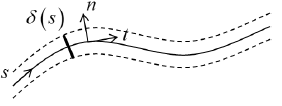
\includegraphics[width=0.5\linewidth]{figures/screenshot012}
\end{figure}
In termini numerici, se si esprime l'altezza del dente - e quindi l'addendum - come un prodotto $km$, poiché tra piano frontale e piano normale cambia il modulo, varierà giocoforza anche questo coefficiente, ma \underline{attenzione} il dente non è che sporge di più o sporge di meno, cambiano soltanto i riferimenti. 

Per cui sul piano normale si avrà $k_n = 1$ - la dentiera sporge di una quantità unitaria per avere il proporzionamento modulare unificato - mentre su quello frontale si avrà $k_f = k$ riportato come segue 
\[k = \dfrac{a}{m} = \dfrac{a\cos\alpha}{m_n} = k_n\cos\alpha\]
Dal punto di visti dalle sporgenze di dice che sul piano frontale il dente è "ribassato" anche se  l'altezza effettiva e la sporgenza dalla primitiva sono le stesse, sono grandezze espresse secondo moduli diversi. \newline 

\textbf{Tutte le grandezze relative alle ruote dentate elicoidali d'ora in poi saranno sempre espresse in funzione di $m_n$} \newline 

Lo spessore del dente, anche se è una misura d'arco, si può scrivere sempre come 
\[s = \dfrac{s_n}{\cos\alpha}\]
Il numero minimo di denti intagliabile per accoppiamento ruota-dentiera è sempre espresso come 
\[z_{min} = \dfrac{2k'}{\sin^2\theta}\]
Tuttavia $k'$ è in relazione ad $\alpha$ come si è visto poco sopra, mentre $\theta$ è preferibile scriverlo in funzione delle grandezze normale, quindi $\theta_n$ angolo d'attacco della dentiera, allora dalla seguente relazione
\[\tan\theta_n = \tan\theta\cos\alpha\]
\[\dfrac{\sin\theta_n}{\sqrt{1-\sin^2\theta_n}} = \dfrac{\sin\theta}{\sqrt{1-\sin^2\theta}}\cos\alpha\]
\[\dfrac{\sin^2\theta_n}{1-\sin^2\theta_n} = \dfrac{\sin^2\theta}{1-\sin^2\theta}\cos^2\alpha\]
Se si considerano piccole variazioni di $\theta, \theta_n$, allora si può scrivere con buona approssimazione 
\[1-\sin^2\theta_n \approx 1-\sin^2\theta\] 
Per cui
\[\sin^2\theta_n = \sin^2\theta\cos^2\alpha\]
Infine, il numero minimo di denti reale si può scrivere così come 
\[z_{min} = \dfrac{2k_n}{\sin^2\theta_n}\cos^3\alpha\]
Questa relazione altro non che che il prodotto tra il numero di denti minimo intagliabile senza interferenza $\dfrac{2k_n}{\sin^2\theta_n}$ applicato ora al piano normale, ovvero il minimo numero di denti fittizi ottenibili con $k_n = 1, \theta_n = 20^\circ$.
\begin{figure}[H]
	\centering
	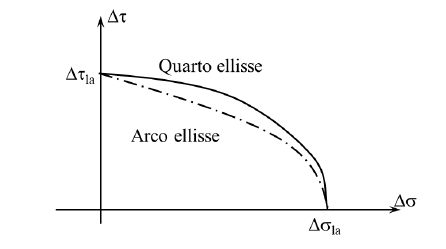
\includegraphics[width=0.5\linewidth]{figures/screenshot013}
	\label{fig:screenshot013}
\end{figure}
\end{adjustwidth}

\subsection{Relazione tra $\alpha$, $\alpha_f$, $\theta_n$}
\begin{adjustwidth}{2in}{}	
	Finora era disponibile la seguente relazione 
	\[\tan\alpha_f = \tan\alpha\cos\theta\]
	Solitamente tale angolo è da ricavare a posteriori perché in partenza si ha sempre $\theta_n$.
	
	Sarebbe quindi utile una relazione che leghi l'angolo d'elica sulla fondamentale, all'angolo d'elica normale all'angolo di pressione normale. 
	Dall'ultima relazione scritta si può passare alla cotangente
	\[\cot^2\alpha_f = \dfrac{\cot^2\alpha}{\cos^2\theta}\]
	In cui si possono sostituire le seguenti relazioni
	\[\begin{dcases}
		\dfrac{1}{\cos^2\theta} = \dfrac{\sin^2\theta+\cos^2\theta}{\cos^2\theta} = 1+\tan^2\theta = 1 + \dfrac{\tan^2\theta_n}{\cos^2\alpha}\\
	\cot^2\alpha_f = \cot^2\alpha\left(1+\dfrac{\tan^2\theta_n}{\cos^2\alpha}\right) = \cot^2\alpha\left(\dfrac{\cos^2\alpha+\tan^2\theta_n}{\cos^2\alpha}\right) = \dfrac{\cos^2\alpha + \tan^2\theta_n}{\sin^2\alpha}\\
	\dfrac{1}{\sin^2\alpha_f} = 1 + \cot^2\alpha_f = 1 + \dfrac{\cos^2\alpha+\tan^2\theta_n}{\sin^2\alpha} = \dfrac{1+\tan^2\alpha_n}{\sin^2\alpha} = \dfrac{1}{\sin^2\alpha\cos^2\theta_n}
	\end{dcases}\]
	Infine si ottiene 
	\[\sin^2\alpha_f = \sin^2\alpha\cos^2\theta_n\]
\end{adjustwidth}
\newpage
\section{Correzione}
\begin{adjustwidth}{2in}{}
	E se gli strisciamenti non vengono verificati?
	
	La correzione si potrà comunque fare anche per le ruote dentate a denti elicoidali elicoidali, con l'accortezza di sapere che sta cambiando l'importa del dente sulla dentiera, anche se cinematicamente è sempre lo stesso meccanismo. 
	
	La correzione in questo caso prevede la distinzione tra piano normale e piano frontale: \textbf{la correzione} $x, x'$ \textbf{si applica sul piano normale}. \newline 
	
	Lo spessore del dente cambia con questa legge 
	\[s_n = \dfrac{\pi m_{0n}}{2} + 2xm_{0n}\tan\theta_{0n}\]
	la stessa vista per le ruote dentate a denti dritti solo che si applicherà allo spessore sul piano normale. \newline 
	
	La scelta dei coefficienti di correzione non varia rispetto a quella adoperata per i denti dritti. Facendo attenzione ad entrare col numero di denti FITTIZIO. \newline 
	
	Con la correzione l'angolo di pressione di funzionamento varia perché varia l'interasse. 
	
	La relazione era questa 
	\[\ev\theta = \ev\theta_0 + 2\tan\theta_0\dfrac{x+x'}{z+z'} = \ev\theta_0 + \dfrac{2\tan\theta_{0n}}{\cos\alpha}\dfrac{x_f+x_f'}{z+z'}\]
	Tale relazione tuttavia si basa sulla forma del dente ad evolvente, quindi in questo caso è necessario riferirla al piano frontale, ponendo semplicemente 
	\[x_f = x\cos\alpha \qquad x_f'=x'\cos\alpha\]
	Sostituendo queste relazioni in quella vista sopra si ha
\begin{equation}\label{eq:evtheta}
		\ev\theta = \ev\theta_0 + 2\tan\theta_{0n}\dfrac{x+x'}{z+z'}
\end{equation}
	\textbf{ATTENZIONE}
	\begin{itemize}
		\item $\theta_{0n}$ è l'angolo d'attacco della dentiera;
		\item $\theta_0$  è l'angolo sul piano frontale di taglio qualora non ci fosse una variazione di interasse, ovvero la proiezione sul piano frontale dell'angolo d'attacco della dentiera. 
		\item $\theta$ è l'angolo di pressione, l'inclinazione del piano dei contatti. 
	\end{itemize}
	A cascata si possono così aggiornare tutte le grandezze in gioco
	\[m = m_0\dfrac{\cos\theta_0}{\cos\theta}\]
	\[\begin{dcases}
		R-R_0 = \eta m_{0n} = \dfrac{z}{2}\left(\dfrac{\cos\theta_0}{\cos\theta}-1\right)\dfrac{m_0n}{\cos\alpha} \\
		R'-R_0' = \eta m_{0n} = \dfrac{z'' }{2}\left(\dfrac{\cos\theta_0}{\cos\theta}-1\right)\dfrac{m_0n}{\cos\alpha} \\
	\end{dcases}\]
	\[I = \dfrac{z+z'}{2}\dfrac{\cos\theta_0}{\cos\theta}\dfrac{m_{0n}}{\cos\alpha} \qquad \varepsilon = \varepsilon_d + \dfrac{b\tan\alpha}{p}\]
	Anche qui dovrà essere effettuato la verifica tra addendum auspicato e addendum effettivo 
	\[a = u'- 0.25m_{0n} = (1-x'+\eta')m_{0n} \qquad a' = u- 0.25m_{0n} = (1-x+\eta)m_{0n}\]
\end{adjustwidth}
%\newpage
\section{Spinte sugli alberi}
\begin{adjustwidth}{2in}{}	
	Il profilo del dente si tocca con il suo coniugato lungo una linea che si svolge in direzione perfettamente assiale per la ruota dentata a denti dritti e secondo un'elica per ruote dentate a denti elicoidali. 
	
	L'approssimazione fatta per le ruote dentate a denti dritti si ripete anche in questo caso:
	\begin{enumerate}
		\item Si sta considerando la forza come risultante della distribuzione di pressione lungo la linea di contatto.
		
		In realtà si ha istante per istante una forza per unità di lunghezza che si considera condensata in un punto ubicato esattamente in mezzeria della larghezza di fascia. \newline 
		
		Nelle ruote dentate elicoidali le forze sono sì sbilanciate (figura \ref{fig:screenshot006}) ma è vero anche che ci sono molti più denti in presa rispetto alla ruote dentate a denti dritti. 
		
		\item Avere più denti in presa mitica l'effetto di sbilanciamento delle forze per le ruote dentate elicoidali. 		
	\end{enumerate}
	Queste approssimazioni ai fini del calcolo delle spinte sugli alberi sono totalmente ininfluenti. \newline 
	
	Le componenti di forza sono 3. 
	\begin{figure}[H]
		\centering
		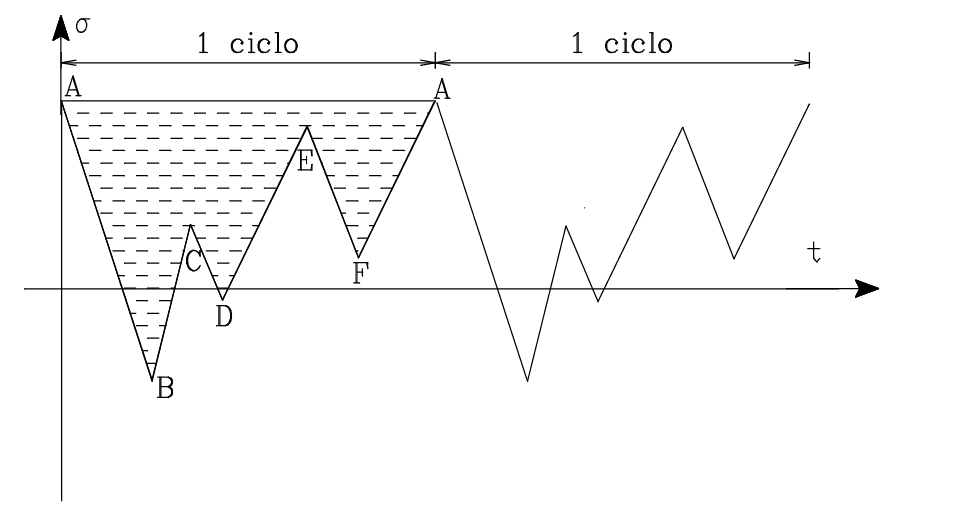
\includegraphics[width=0.2\linewidth]{figures/screenshot014}
		\caption{Il dente scambia normalmente alla superficie}
		\label{fig:screenshot014}
	\end{figure}
	Ci saranno
	\begin{itemize}
		\item Una componente assiale
		\[N\sin\alpha_f\]
		\item Una componente radiale nel piano frontale 
		\[N\cos\alpha_f\]
		Questa componente avrà a sua volta 
		\begin{itemize}
			\item Una componente radiale 
			\[N\cos\alpha_f\sin\theta\]
			\item Una componente circonferenziale/spinta utile
			\[N\cos\alpha_f\cos\theta\]
		\end{itemize}
		
	\end{itemize}
	
	\textbf{Remainder}: $\theta$ è l'angolo di pressione sul piano frontale, quello ovvero ottenuto dall'equazione (\ref{eq:evtheta}), mentre $\alpha_f$ è l'angolo d'elica sulla fondamentale. 
	
	Siccome non è comodo da usare questo $\alpha_f$, viene utilizzato quello sulla primitiva $\alpha$.
	
	Si ottengono così, infine
	\begin{itemize}
		\item \textbf{Componente circonferenziale/tangenziale/spinta utile}
		\[Q = N\cos\alpha_f\cos\theta=\dfrac{M_T}{R}\]
		\item \textbf{Componente assiale}
		\[F_A = Q\tan\alpha\]
		\item \textbf{Componente radiale}
		\[F_R = Q\tan\theta\]		
	\end{itemize} 
	Solitamente $\alpha=(20\div25)^\circ$. 
\begin{figure}[H]
	\centering
	\label{fig:screenshot015}
	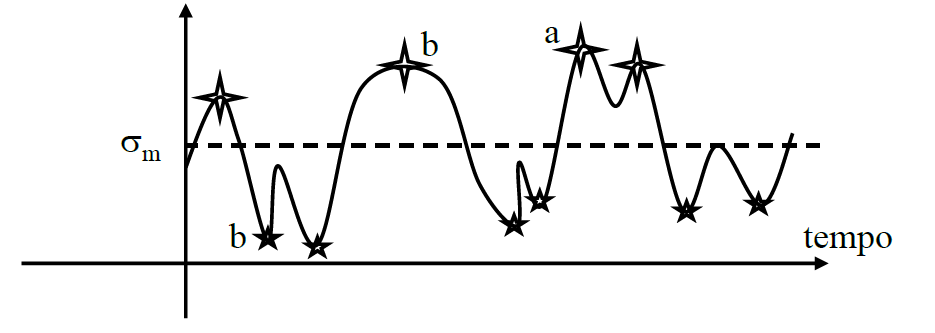
\includegraphics[width=0.5\linewidth]{figures/screenshot015}
	\caption{}
\end{figure}
Alla luce di ciò, sapendo che ruota condotta e ruota motrice devono avere eliche opposte, allora il riduttore vedrà - se necessario angolo di rinvio - due accoppiamenti di ruote dentate, vuol dire che l'albero di rinvio alloggia contemporaneamente la condotta del primo ingranaggio e la motrice del secondo, siccome si era detto che il grosso svantaggio delle dentature elicoidali sono le spinte assiali, come si sceglie l'elica della condotta del primo ingranaggio rispetto alla motrice del secondo? 

Eliche opposte spaccano i cuscinetti. \newline

Considerando l'albero di rinvio, le forze circonferenziali che agiscono sulla prima (condotta) e sulla seconda (conduttrice) sono equiverse: a parità di rotazione una è concorde ed una è discorde, quelle componenti sono esattamente le componenti circonferenziali di una forza normale al profilo.
\newpage
Le eliche della figura \ref{fig:screenshot015} sono concordi, solo in questo modo le forze assiali possono bilanciarsi! 
\begin{figure}[H]
	\centering
\begin{tikzpicture}[>=latex]
	%%%	Help Lines
%	\draw [thin, help lines] (0,0) grid (10,10);
%	\foreach \x in {0,...,10}
%	\draw (\x cm,1pt) -- (\x cm,-1pt) node[anchor=north] {$\x$};
%	\foreach \y in {0,...,10}
%	\draw (1pt,\y cm) -- (-1pt,\y cm) node[anchor=east] {$\y$};
	%%%	Disegno	
	% Motrice
	\draw[thick] (0,0) rectangle (3,5);
	\draw[thick, red] (0,1) -- (3,4);
	
	\tkzDefPoints{1.5/2.5/A, 0/1/B, 3/4/C}
	\tkzDefLine[orthogonal=through A](C,B) \tkzGetPoint{X1}
	
	\draw[thick, ->] (A) -- (X1) node[right] {$F_N$};
	\draw[thick, ->] (A) -- (1.5, -0.5) node[below] {$F_C$};
	\draw[thick, ->] (A) -- (4.5, 2.5) node[below] {$F_A$};
	\node[rectangle] at (1.5, 6.25) {Motrice};
	
	% Condotta
	\draw[thick] (7,0) rectangle (10,5);
	\draw[thick, red] (7,1) -- (10,4);
	
	\tkzDefPoints{8.5/2.5/A1, 7/1/B1, 10/4/C1}
	\tkzDefLine[orthogonal=through A1](B1,C1) \tkzGetPoint{X11}
	
	\draw[thick, ->] (A1) -- (X11) node[right] {$F_N$};
	\draw[thick, ->] (A1) -- (8.5, 5.5) node[above] {$F_C$};
	\draw[thick, ->] (A1) -- (5.5, 2.5) node[below] {$F_A$};
	\node[rectangle] at (8.5, 6.25) {Condotta};
	
\end{tikzpicture}
\caption{Eliche dello stesso verso}
\end{figure}
 
 
\begin{figure}[H]
	\centering
	 \begin{tikzpicture}[>=latex]
 	%%%	Help Lines
% 	\draw [thin, help lines] (0,0) grid (10,10);
% 	\foreach \x in {0,...,10}
% 	\draw (\x cm,1pt) -- (\x cm,-1pt) node[anchor=north] {$\x$};
% 	\foreach \y in {0,...,10}
% 	\draw (1pt,\y cm) -- (-1pt,\y cm) node[anchor=east] {$\y$};
 	%%%	Disegno	
 	% Motrice
 	\draw[thick] (0,0) rectangle (3,5);
 	\draw[thick, red] (0,1) -- (3,4);
 	
 	\tkzDefPoints{1.5/2.5/A, 0/1/B, 3/4/C}
 	\tkzDefLine[orthogonal=through A](C,B) \tkzGetPoint{X1}
 	
 	\draw[thick, ->] (A) -- (X1) node[right] {$F_N$};
 	\draw[thick, ->] (A) -- (1.5, -0.5) node[below] {$F_C$};
 	\draw[thick, ->] (A) -- (4.5, 2.5) node[below] {$F_A$};
 	\node[rectangle] at (1.5, 6.25) {Motrice};
 	
 	% Condotta
 	\draw[thick] (7,0) rectangle (10,5);
 	\draw[thick, red] (7,4) -- (10,1);
 	
 	\tkzDefPoints{8.5/2.5/A1, 7/4/B1, 10/1/C1}
 	\tkzDefLine[orthogonal=through A1](B1,C1) \tkzGetPoint{X11}
 	
 	\draw[thick, ->] (A1) -- (X11) node[right] {$F_N$};
 	\draw[thick, ->] (A1) -- (8.5, 5.5) node[above] {$F_C$};
 	\draw[thick, ->] (A1) -- (11.5, 2.5) node[below] {$F_A$};
 	\node[rectangle] at (8.5, 6.25) {Condotta};
 	
 \end{tikzpicture}
 \caption{Eliche di verso opposto}
\end{figure}

	










		
		
		
		





































\newpage
\textbf{{\LARGE NOTE}}
%	\vfill
%	\begin{tcolorbox}[height=4.5cm]
%		This box has a height of 4.5cm.
%	\end{tcolorbox}

%DA DECOMMENTARE PER AVERE LA VERSIONE STAMPABILE A DUE PAGINE 	
%	\newpage
%		\null
%		\vfill
%\begin{tcolorbox}[height=4.5cm]
%	This box has a height of 4.5cm.
%\end{tcolorbox}
%		
\end{adjustwidth}
\end{document}